% !TEX root = ../stellar-notes.tex

Much of these notes will be concerned with the essential {\it physics} of stars.
We will focus on the questions: What determines the structure and evolution of stars of varied initial properties? What are the end states of stars? and How do stars affect cosmic chemical evolution?

We shall see that much of the salient physics of stars separates into two broad categories: {\it macrophysics} and {\it micriphysics}, the former characterized by, e.g., the mechanical equations of stellar structure, and the latter characterized by, e.g., the physics of nuclear reactions.
We will also see that these two limits, the large and small, are fundamentally coupled and that, in large part, the macrophysical equations are simply a continuum limit of the governing microphysical equations (analogous to how classical physics is a particular limit of quantum physics).
In an extremely reductionist sense, a star's life can be described as a struggle between the inexorable inward pull of its own gravity and the competing outward push of various forms of pressure, the latter generated by different types of microphysical processes.
As a star evolves and changes, the physics that dominates the generation of this outward pressure changes frequently, altering the essential character of the star in important ways.
But gravity remains every constant in its pull, seeking to make anything and everything it can into a black hole. \footnote{anthropomorphism: {\it noun}, the attribution of human characteristics or behavior to a animal, object, or force of nature.}

Before digging into the physics, it is useful to review some observational and nomenclatural aspects of stars.
Figure \ref{f.hubblestars} shows a field of stars in Sagitarius as imaged by the Hubble Space Telescope (HST).
These stars clearly span a range in color, from red to blue, and brightness.
Also apparent is that the bluer stars appear brighter.
Stars are classified according to their {\it spectral type}, denoted by letters OBAFGKM.
We now know that this seemingly random arrangement of letters reflects the effect temperatures at which stars radiate.
The original spectral classification scheme developed at Harvard Observatory by Annie Jump Cannon was based solely on spectral features (Balmer lines) and was, indeed, alphabetical.
Once it was understood that different Balmer lines appear as a function of effective temperature, the spectral classes were rearranged in order of decrease temperature.

\begin{figure}[ht!]
  \centering
  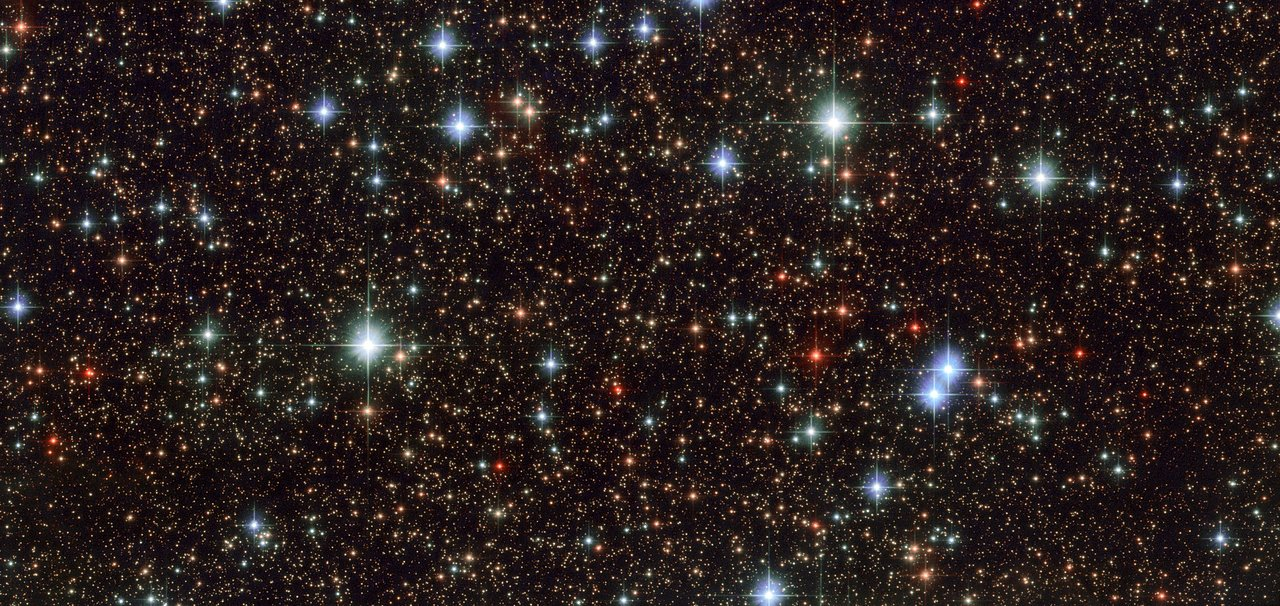
\includegraphics[width=0.9\textwidth]{prelim/hubble_friday_06172016}
  \caption{Hubble Space Telescope image of stars in the constellation Sagitarius. {\it Image credit: NASA/ESA.}}\label{f.hubblestars}
\end{figure}

Table \ref{t.spectralclass} lists the modern Harvard spectral types and some of their salient properties, including Main Sequence mass, radius, and luminosity.
Immediately apparent is the strong dependence of all these properties on the mass of the stars.
The most important parameter in determining the evolution of a star is its initial mass, usually termed as the Zero-age Main Sequence (ZAMS) mass.
But this is not the only important evolutionary parameter.
A stars {\it metallicity}, or content of elements heavier than H and He, as well as the initial angular momentum content and magnetic field strength are also critical.
These latter two are inextricably linked and subject to substantial uncertainties, both in their typical values for stars and in their impact on stellar evolution.
The roles of rotation and magnetic fields in stellar structure and evolution will be explored in Chapter \ref{ch.rotation}.
Another critical component in determining the fate of a star, particularly a massive star, is whether or not it has a close binary companion.
Important aspects of binarity will be discussed in Chapter \ref{ch.binaries}.


\begin{table}[hbt]
  \caption{The Modern Harvard Stellar Spectral Types}\label{t.spectralclass}
  \begin{tabular}{c|p{0.2\textwidth}p{0.2\textwidth}p{0.2\textwidth}p{0.2\textwidth}}
  \hline
  Type & Effective temperature & Main sequence mass & Main sequence radius & Main sequence bolometric luminosity \\
  \hline\hline
  O & $\gtrsim30,000$ K & $\gtrsim16\ M_\sun$ & $\gtrsim6.6\ R_\sun$ & $\gtrsim30,000\ L_\sun$ \\
  B & 10,000--30,000 K & 2.1--16 $M_\sun$ & 1.8--6.6 $R_\sun$ & 25--30,000 $L_\sun$ \\
  A & 7,500--10,000 K & 1.4--2.1 $M_\sun$ & 1.4--1.8 $R_\sun$ & 5--25 $L_\sun$ \\
  F & 6,000--7,500 K & 1.04--1.4 $M_\sun$ & 1.15--1.4 $R_\sun$ & 1.5--5 $L_\sun$ \\
  G & 5,200--6,000 K & 0.8--1.04 $M_\sun$ & 0.96--1.15 $R_\sun$ & 0.6--1.5 $L_\sun$ \\
  K & 3700--5200 K & 0.45--0.8 $M_\sun$ & 0.7--0.96 $R_\sun$ & 0.08--0.6 $L_\sun$ \\
  M & 2400--3700 K & 0.08--0.45 $M_\sun$ & $\lesssim$0.7 $R_\sun$ & $\lesssim$0.08 $L_\sun$ \\
  \hline
  \end{tabular}
\end{table}

The spectral classifications in Table \ref{t.spectralclass} are supplemented by {\it luminosity classes}, denoted by Roman numerals, with ``I'' being the brightest supergiants and ``V'' being main sequence stars.
The spectral classes are also typically augmented by and additional Arabic numeral further specifying the star's precise effective temperature.
So, for example, our Sun is a ``G2 V,'' being a main sequence star with an effective temperature of 5770 K.

\begin{figure}[htb]
  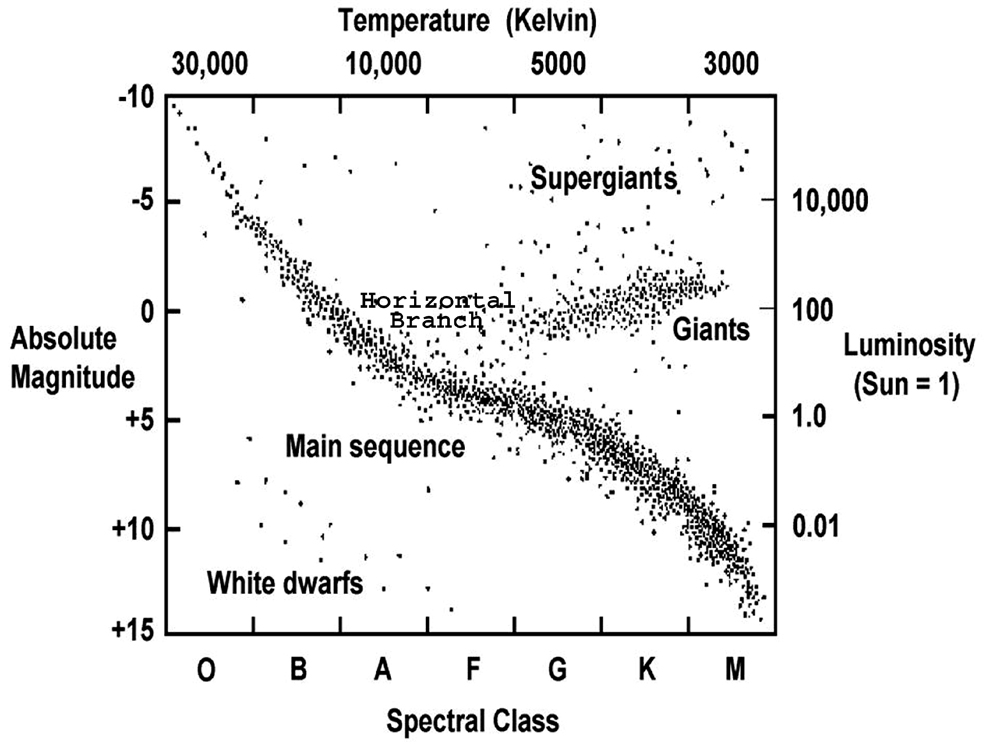
\includegraphics[width=0.9\textwidth]{prelim/HR_diagram}
  \caption{Example HR diagram for a subset of stars in the Milky Way.}
  \label{f.hrd}
\end{figure}

The principle graphical tool for understanding stellar evolution is the {\it Hertzprung-Russel (HR) diagram}.
Stars are placed on the HR diagram depending on their effective temperature (i.e., spectral type) and their absolute luminosity.
An example HR diagram is shown in Figure \ref{f.hrd}.
Observationally, it is generally easier to produce a {\it color-magnitude} diagram in which the absolute magnitude in a given broadband filter is plotted against the {\it color}, usually the difference of magnitudes between two broadband filters.
